% !Mode:: "TeX:UTF-8"
\documentclass[proposal]{skythesis}
%\renewcommand{\encodingdefault}{T1}
%\renewcommand{\familydefault}{cmbr}
\graphicspath{{figures/}}  % 定义所有的eps文件在 figures 子目录下
\begin{document}

% !Mode:: "TeX:UTF-8"
%%============================================================
%% 中文封面

\thispagestyle{empty}
\pdfbookmark[-1]{\zjuttitlec}{zjutthesiscover}
\phantomsection \label{zjutthesiscover}
\vspace*{4mm}
% 校名
\begin{center}
   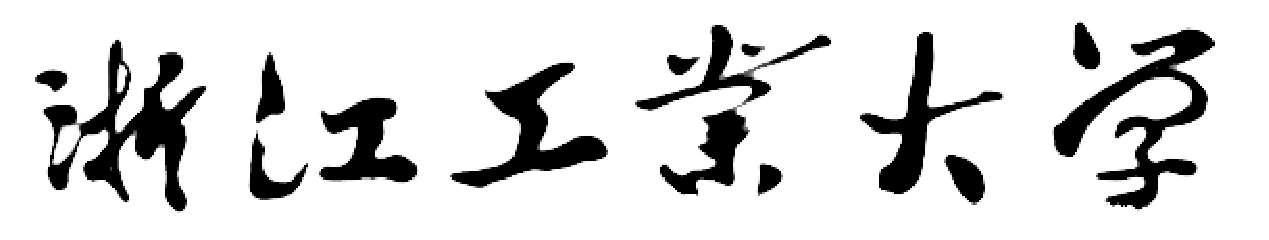
\includegraphics[width=98.40mm]{figures/zjut}
\end{center}
\vspace*{12mm}
\centerline{\songti\yihao{本科毕业设计说明书(论文)}}
\vspace*{8mm}
\centerline{\songti\xiaoer\textbf{(\zjutgrade\ 届)}}
\vspace*{7mm}
% 校徽
\begin{center}
  
\includegraphics[width=27.3mm]{figures/zjutlogo}
\end{center}

\vspace*{0.0mm}
\renewcommand{\arraystretch}{1.0}
\hspace*{12mm} 
{\songti\erhao{论文题目}}
\hspace{6mm} 
\begin{minipage}[t]{85mm} % 这里建议自行微调
    \linespread{1.1}{\songti\xiaoer\CJKunderline*{\zjuttitlec}}
\end{minipage}
\vspace*{1mm}
\begin{center}
    \setlength{\arrayrulewidth}{0.5pt}
    {\songti\sihao
        \renewcommand{\arraystretch}{1}
        \begin{tabular}{lc}
            作者姓名\qquad &  \zjutauthornamec \\ \cline{2-2}
            指导教师\qquad &  \zjutmentorc\\ \cline{2-2}
            \\
            学科(专业)\qquad &  \zjutmajor \\ \cline{2-2}
            所在学院\qquad &  \zjutcollegec \\ \cline{2-2}
            提交日期\qquad & \zjutsubmitteddatee \\ \cline{2-2}
        \end{tabular}
    }
\end{center}

      % 封面

\frontmatter

\begingroup % 在组内的chapter不换行

\let\cleardoublepage\relax
%% !Mode:: "TeX:UTF-8"
%% 中文摘要
\begin{abstractc}
\begin{center}
{
\xiaosi
\vspace{1em}

 学生姓名:\extt[2.8em]{\skyauthornamec}\hspace{20mm} 指导老师:\extt[6.4em]{\skymentorc}

\skyschoolc\skycollegec}

{\xiaosan\bf\vbox{} \heiti {摘\quad 要}}
\vspace{-1cm}
\end{center}

{\onehalfspacing \sihao \songti \indent

\input{preface/mainc.txt}
}
\end{abstractc}     % 中文摘要
%% !Mode:: "TeX:UTF-8"
%% 英文摘要
\begin{abstracte}
\begin{center}
\vspace{1em}
{\xiaosi \onehalfspacing
 Author: \Skyauthorc\hspace{20mm} Mentor: \Skymentorc

\Skycollegec, \Skyschoolc

{\xiaosan\bf\vbox{} Abstract}
}
\end{center}

{\onehalfspacing
\indent \sihao \input{preface/maine.txt}}
\end{abstracte}
     % English Abstract
%{\singlespacing\tableofcontents           % 中文目录
%\listoffigures             % 图目录
%\pagenumbering{Roman}
%\listoftables              % 表目录
%\pagenumbering{Roman}


%%%%%%%%%% 正文 %%%%%%%%%%
\mainmatter
\makeatletter
% !Mode:: "TeX:UTF-8"
\chapter{课题研究背景与意义}
掀起各国企业学习和运用的热潮。作为IE技术的基础运用,工作研究是最基本的技术,也是其他新兴IE技术运用的基础。企业在学习各种新的IE技术和\cite{2007}

\begin{equation}
\label{equaa5}
\iiint_1^1\frac{f(x)}{\sqrt{1-x^2}}dx = \frac{\pi}{n}\sum_{k=1}^nf(cos\frac{2k-4}{2n})+\frac{\pi}{2^{2n-1}(2n)!}f^{(2n)}(\theta)+max+\max
\end{equation}

张图片独自占一行的插入形式如\eqref{equaa5}~所示。

\chapter{课题研究的目标}
掀起各国企业学习和运用的热潮。作为IE技术的基础运用,工作研究是最基本的技术,也是其他新兴IE技术运用的基础。企业在学习各种新的IE技术和\cite{2007}

\begin{equation}
\label{equaa6}
\iiint_1^1\frac{f(x)}{\sqrt{1-x^2}}dx = \frac{\pi}{n}\sum_{k=1}^nf(cos\frac{2k-4}{2n})+\frac{\pi}{2^{2n-1}(2n)!}f^{(2n)}(\theta)+max+\max
\end{equation}

张图片独自占一行的插入形式如\eqref{equaa6}~所示。
% !Mode:: "TeX:UTF-8"
\chapter{课题研究的主要内容}
\section{研究对象简介}

\section{研究对象存在的问题}

% !Mode:: "TeX:UTF-8"
\chapter{采用的关键技术及技术路线}
\section{关键技术}

\section{关键路线}


% !Mode:: "TeX:UTF-8"
\chapter{计划进度}
毕业设计的时间安排如\reft{tab:myschedule}所示。

\begin{table}[H]
  \centering
  \caption{毕业设计进度计划安排}
    \begin{tabular}{cccl}
    \toprule
    \multicolumn{3}{c}{\textbf{起 止 时 间}} & \multicolumn{1}{c}{\textbf{阶  段  任  务  要  点}} \\
    \midrule
    \textbf{2013.12.01} & --    & \textbf{2014.02.01} & 外文翻译、文献综述和开题报告初稿 \\
    \textbf{2014.02.21} & --    & \textbf{2014.03.15} & 完善外文翻译、文献综述和开题报告 \\
    \textbf{2014.03.15} & --    & \textbf{2014.03.31} & 毕业设计调研 \\
    \textbf{2014.04.01} & --    & \textbf{2014.04.25} & 论文初稿 \\
    \textbf{2014.04.26} & --    & \textbf{2014.05.05} & 论文二稿 \\
    \textbf{2014.05.06} & --    & \textbf{2014.05.20} & 论文三稿 \\
    \textbf{2014.05.21} & --    & \textbf{2014.06.10} & 定稿、准备答辩 \\
    \bottomrule
    \end{tabular}%
  \label{tab:myschedule}%
\end{table}%


%%%%%%%%%% 参考文献 %%%%%%%%%%
\bibliography{references/reference}
\nocite{*}    % 若将此命令屏蔽掉,则未引用的文献不会出现在文后的参考文献中。
\makeatother

\backmatter
\endgroup % 组结束


%%%%%%%%%% 致谢 %%%%%%%%%%
%% !Mode:: "TeX:UTF-8"

%\titlecontents{chapter}[2em]{\vspace{.5\baselineskip}\wuhao\hei}
%{\prechaptername\CJKnumber{\thecontentslabel}\postchaptername\qquad}{}
%{\hspace{.5em}\titlerule*[10pt]{$\cdot$}\wuhao\contentspage}
\chapter{致谢}

浙江工业大学本科生毕业论文~\LaTeX~模板主要参考以下内容:
\begin{itemize}
  \item 天津大学本科生毕业论文
  \item 哈尔滨工业大学~PlutoThesis~硕博士学位论文模板
  \item 武汉理工大学学位论文~WHUTThesis~模板
  \item 中科院~CASthesis~模板
  \item 浙江大学~cs\_zjut\_theis~模板
  \item 上海交通大学毕业论文Latex模板
\end{itemize}

\vspace*{1em}

衷心感谢导师~XXX~(职称)对本人的精心指导。他/她的言传身教将使我终生受益。

感谢~XXX~教授,以及实验室全体老师和同窗们的热情帮助和支持!




            % 致谢
%\include{body/lit}
%%%%%%%%%% 附录 %%%%%%%%%%
%\appendix
%% !Mode:: "TeX:UTF-8"
%
% XXX refactor 暂时当静态页面处理
% 
\chapter*{\heiti\bfseries{\appendixtitle}}
\chaptermark{\appendixname}
\addcontentsline{toc}{chapter}{\cusongti{\appendixname}}
\phantomsection

\addcontentsline{toc}{section}{附录1 毕业设计文献综述}
\addcontentsline{toc}{section}{附录2 毕业设计开题报告}
\addcontentsline{toc}{section}{附录3 毕业设计外文翻译}
\hspace*{7.0mm}
\hspace*{4.0mm}
\begin{minipage}[t]{95mm}
    \heiti\bfseries{
    \sectionmark{附录1 毕业设计文献综述}
    附录1 毕业设计文献综述

    \vspace*{7.0mm}

    \sectionmark{附录2 毕业设计开题报告}
    附录2 毕业设计开题报告

    \vspace*{7.0mm}

    \sectionmark{附录3 毕业设计外文翻译}
    附录3 毕业设计外文翻译}
\end{minipage}


            % 附录

\end{document}                                  % 结束全文
